\chapter{Resolving technical debt}

\section{Introduction}



\label{chap:fixes}
\section{Navbox}
At the beginning of the semester I verified that the \gls{navbox} worked as it was supposed to.
The only detected error was that \gls{kartverket} had removed the acces key to thei API,
which was resolved by contacting them and asking for a new key with a longer expiration date.

Later, when creating a page for the \gls{navbox} in the \srgui I discovered that the \gls{navbox} was not working as zero data was being received.
The \gls{navbox} had been stored for months in a drawer since the last verification.
Thre potential culprits were identified.

\subsection{Potential cause 1: \jx software}
The first potential culprit is that the \gls{spi} driver, the \gls{spi} \py interface or the \gls{gpio} interface stopped working when the \jx was flashed with the new \gls{os}.

\subsection{Potential cause 2: damage from exessive input voltage}
The \gls{pico} might have been damaged by exessive input voltage from the \gls{stim}.
Revisiting the \gls{navbox} scematics, Figure 27 of the \preproject, and measuring voltages with a multimeter revealed that the \gls{tov} signal from the \gls{stim} was at $5V$.
This is not supported by the \gls{gpio} pins on the \gls{pico}, but it is however not likely that this has caused damage as the \gls{pico} normally can tolerate $5V$ without getting damaged \cite[17]{PicoDatasheet}\cite{aryavoronovaRP20405VLogic2023}
The voltage of digital output signals on the \gls{stim} was still lowered to $3.3V$ according to Table 12-1 in the \gls{stim} datasheet to make sure this is not an issue in the future \cite[118]{safranSTIM300Datasheet}

\subsection{Potential cause 3: damage to hardware}
A third option is that any of the wires on the \gls{navbox} have been damaged.
This appears unlikely as the \gls{navbox} has been stored in a drawer and not used since the last verification, but it is still a possibility.

\subsection{Solution}
After quite a bit of troubleshooting, without finding the cause of the issue, I decided to start restructuring the \gls{navbox} interface.
The current solution have many points of failure and require an intrequite reading interface on the \jx, described in Section 5.4 of the \preproject, and is time consuming to replicate.
As we have got funding to create a second sensor rig, and potential funding of a third one has been discussed, I will have to create at least one more \gls{navbox} interface in the future.
This is why I decided to start restructuring the \gls{navbox} interface to make it easier to replicate and less prone to errors.
The new interface is built on communicating and powering the \gls{navbox} over \gls{usb} instead of \gls{spi} and \gls{gpio}, and communicating between the \gls{navbox} and the \glsps{f9p} over \gls{qwiic}.
This dramatically reduces the number of wires needed, and makes it easier to replicate as shown in Figure \ref{fig:navbox_usb}, compared to Figure 27 of the \preproject.

\begin{figure}[H]
    \centering
    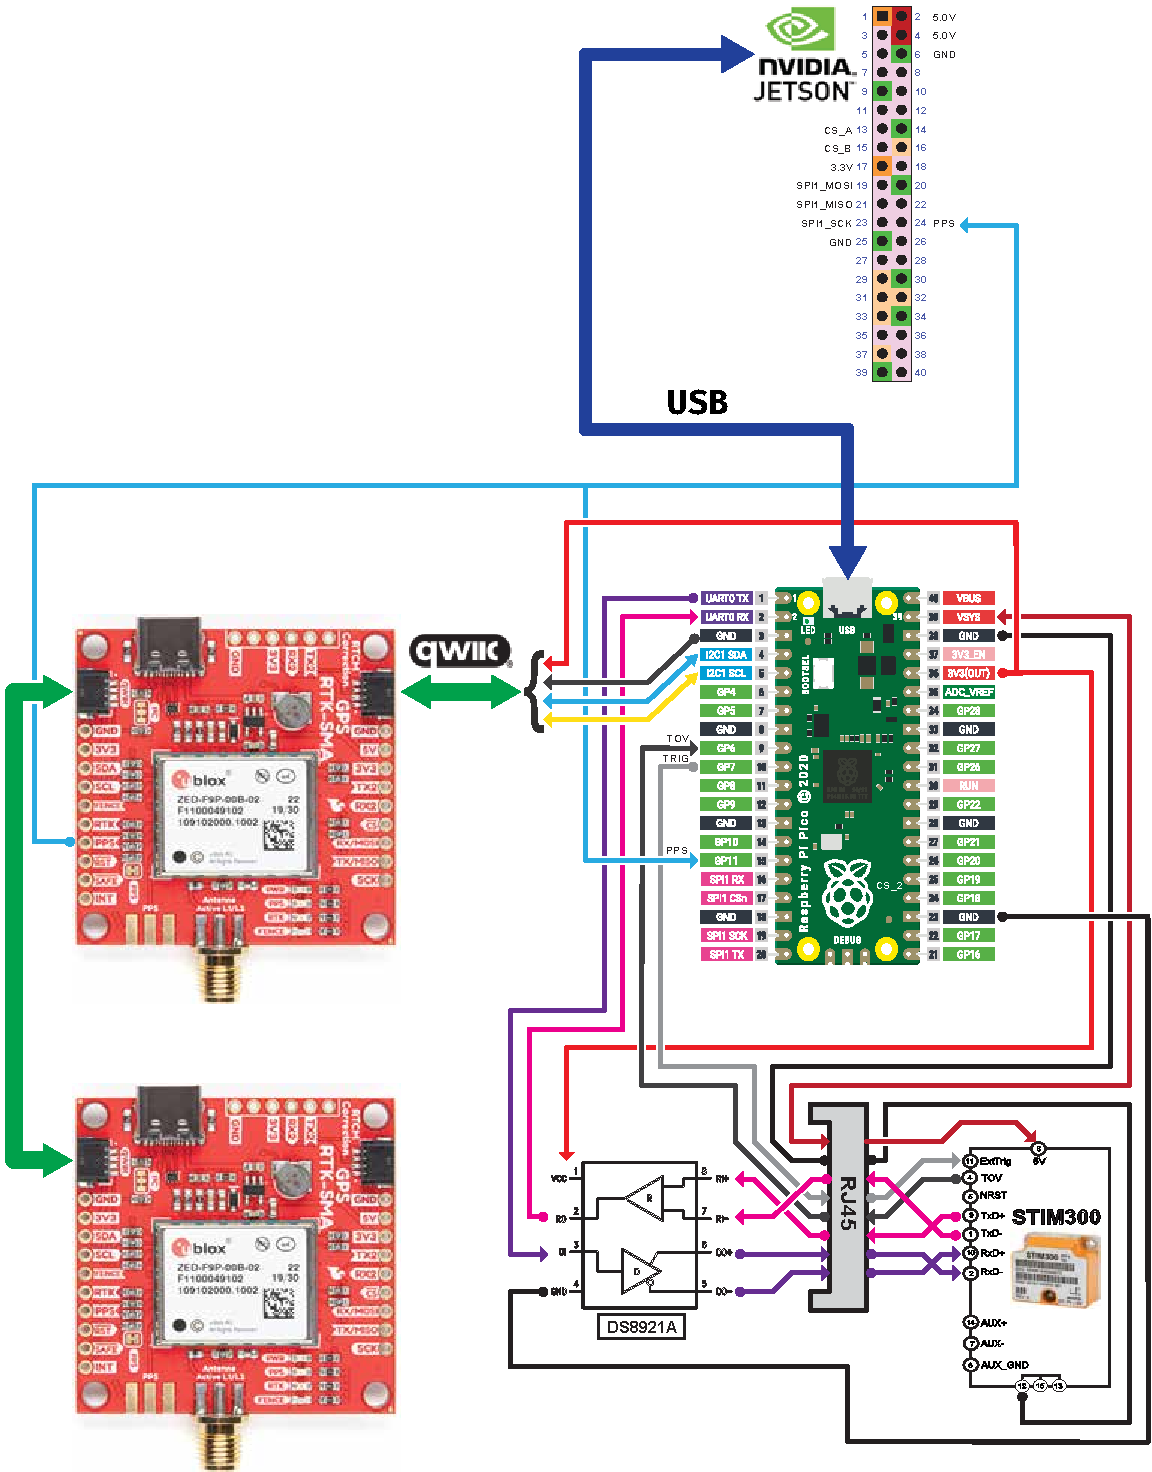
\includegraphics[width=\textwidth]{figures/navbox/navbox_usb.pdf}
    \caption{Scematics of the new \gls{navbox} interface comparet to Figure 27 of the \preproject}
    \label{fig:navbox_usb}
\end{figure}

\subsection{Raspberry Pi Pico USB speed}
The main potential issue with the new proposed setup was that it relies on a quite high \gls{usb} speed between the \gls{pico} and the \jx, as \gls{stim} alone can procude up $124kB/s$ when running at max frequency of $2khz$ \cite[34]{safranSTIM300Datasheet}.
Building on the example code on communicate with the \gls{pico} over \gls{usb}

\subsection{Raspberry Pi Pico Workflow}
By setting \code{PICO_STDIO_USB_RESET_MAGIC_BAUD_RATE} to $1200$ in the \gls{cmake} file it is possible to get the \gls{pico} into boot mode without manually pressing the \code{bootsel} button and reconnecting it \cite{hermannswAnswerSettingUsb2021}.
As the development of the \gls{pico} code also is done in a Docker container inside \gls{wsl}

on a Windows host, and the \gls{pico} is flashed from a docker container, a small \py server was created to make the development process on the \gls{pico} easier.
A small \py server was created to make the development process on the \gls{pico} easier.

As this requires reconnecting it and manually copying the compiled code to the \gls{pico} I decided to make a small pipeline that automates this process.
A small Python server runs on the Windows host and flashes the \gls{pico} when it receives compiled code from a docker container.
After the \gls{pico} has been flashed the server opens a serial connection and acts as an interface between the \gls{pico} and programs running in docker container.




